\section{BPSK Modulation}
\label{sec:bpsk}

\subsection{Objective}
To study passband digital communication technique BPSK and
Calculate the BER of BPSK modulated signal.

\subsection{Theory}
Binary Phase Shift Keying (BPSK) is a digital modulation technique
in which the information is transmitted by changing the phase of a
carrier wave. The phase of the carrier wave is shifted
from 0 to 180 degrees for a binary 1 and from 0 to 360 degrees
for a binary 0.

BPSK is widely used in various applications such as satellite communication,
wireless communication, and digital audio broadcasting due
to its simplicity and robustness to noise.

The BER for BPSK can be calculated as follows:

\begin{equation}
    \label{eq:bpsk}
    BER = \frac{1}{2}\, \textnormal{erfc}\left( \frac{E_b}{N_0} \right)
\end{equation}

where $E_b$ is the energy per bit and $N_0$ is the noise power spectral density.

\subsection{MATLAB Code}

\inputminted[fontsize=\footnotesize,autogobble]{matlab}{code/bpsk.m}

\subsection{Output}

\begin{figure}[!htb]
    \centering
    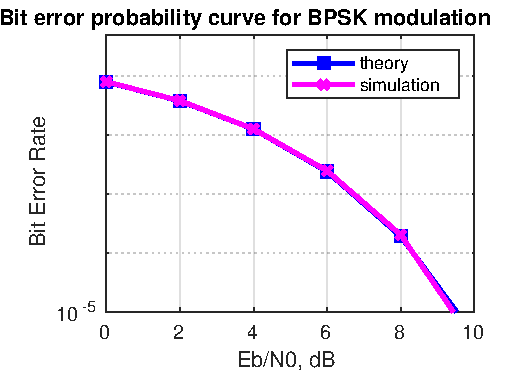
\includegraphics[width=0.7\textwidth]{res/figures/BPSK.pdf}
    \label{output:bpsk}
    \caption{BPSK}
\end{figure}

\pagebreak

\section{BPSK in presence of Noise}
\label{sec:bpsk noise}

\subsection{Objective}
To study the effect of noise on Binary PSK modulation.

\subsection{Theory}
The effect of noise on BPSK modulation can be studied by
adding noise to the modulated signal. The noise can be added
in the form of AWGN or Rayleigh fading.

In the presence of noise, the receiver may make errors in
decoding the signal. To measure the system's performance,
the signal-to-noise ratio (SNR) is used,
and the bit error rate (BER) is calculated to determine
the probability of error in the received data.
The trade-off between the SNR and BER determines the
system's reliability in noisy environments

\subsection{MATLAB Code}

\inputminted[fontsize=\footnotesize,autogobble]{matlab}{code/bpsk_noise.m}

\subsection{Input}

\begin{lstlisting}[language=matlab,backgroundcolor=\color{gray!10}]
Enter the Bit stream: 
[1 0 1 1 0 1]
\end{lstlisting}

\subsection{Output}

\begin{figure}[!htb]
    \centering
    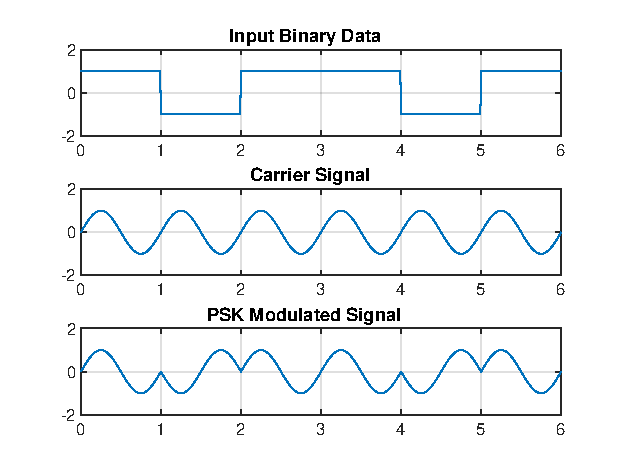
\includegraphics[width=0.8\textwidth]{res/figures/BPSK_noise.pdf}
    \label{output:bpsk noise}
    \caption{BPSK in presence of Noise}
\end{figure}